\documentclass{beamer}
\usepackage[utf8]{inputenc}
\usepackage{subfig}
\usepackage{utopia} %font utopia imported
\usepackage{arabtex}
\usepackage{utf8}
\setcode{utf8}
\usetheme{Madrid}
\usecolortheme{default}

%------------------------------------------------------------
%This block of code defines the information to appear in the
%Title page
\title[Standard Cell] %optional
{Standard Cells, and Physical Only Cells }

\subtitle{in ASIC Design}

\author[Ahmed Abdelazeem] % (optional)
{Ahmed Abdelazeem}
%{A.~B.~Arthur\inst{1} \and J.~Doe\inst{2}}

\institute[ZU] % (optional)
{
	Faculty of Engineering\\
	Zagazig University
}
%{
%	\inst{1}%
%	Faculty of Engineering\\
%	Zagazig University
%	\and
%	\inst{2}%
%	Faculty of Chemistry\\
%	Very Famous University
%}

\date[ZU 2023] % (optional)
{RTL2GDSII Flow, November 2022}

%\logo{
\includegraphics[height=1.5cm]{lion-logo.png}}

%End of title page configuration block
%------------------------------------------------------------



%------------------------------------------------------------
%The next block of commands puts the table of contents at the
%beginning of each section and highlights the current section:

\AtBeginSection[]
{
	\begin{frame}
		\frametitle{Table of Contents}
		\tableofcontents[currentsection]
	\end{frame}
}
%------------------------------------------------------------


\begin{document}
	
	%The next statement creates the title page.
	\frame{\titlepage}
	
	
	%---------------------------------------------------------
	%This block of code is for the table of contents after
	%the title page
	\begin{frame}
		\frametitle{Table of Contents}
		\tableofcontents
	\end{frame}
	%---------------------------------------------------------
	
	
	\section{Standard Cells}
	
	%---------------------------------------------------------
	%Changing visivility of the text
	\begin{frame}
		\frametitle{Introduction}
		\begin{itemize}
			\item \textbf{Standard cells} are a collection of \textcolor {red} {well-defined} and \textcolor {red} {pre-characterized} cells with \textcolor {red} {multi-drive strength} and \textcolor {red} {multi-threshold voltage} cells in the form of a \textcolor {red} {predefined standard cell layout}. 
			\item It also contains a number of physical only cells and a set of library files required by Place and Route (PnR) tool for automatic placement and routing.
			\item Standards cells are highly reusable as it is save lots of ASIC design time.
		\end{itemize}
	\begin{center}
	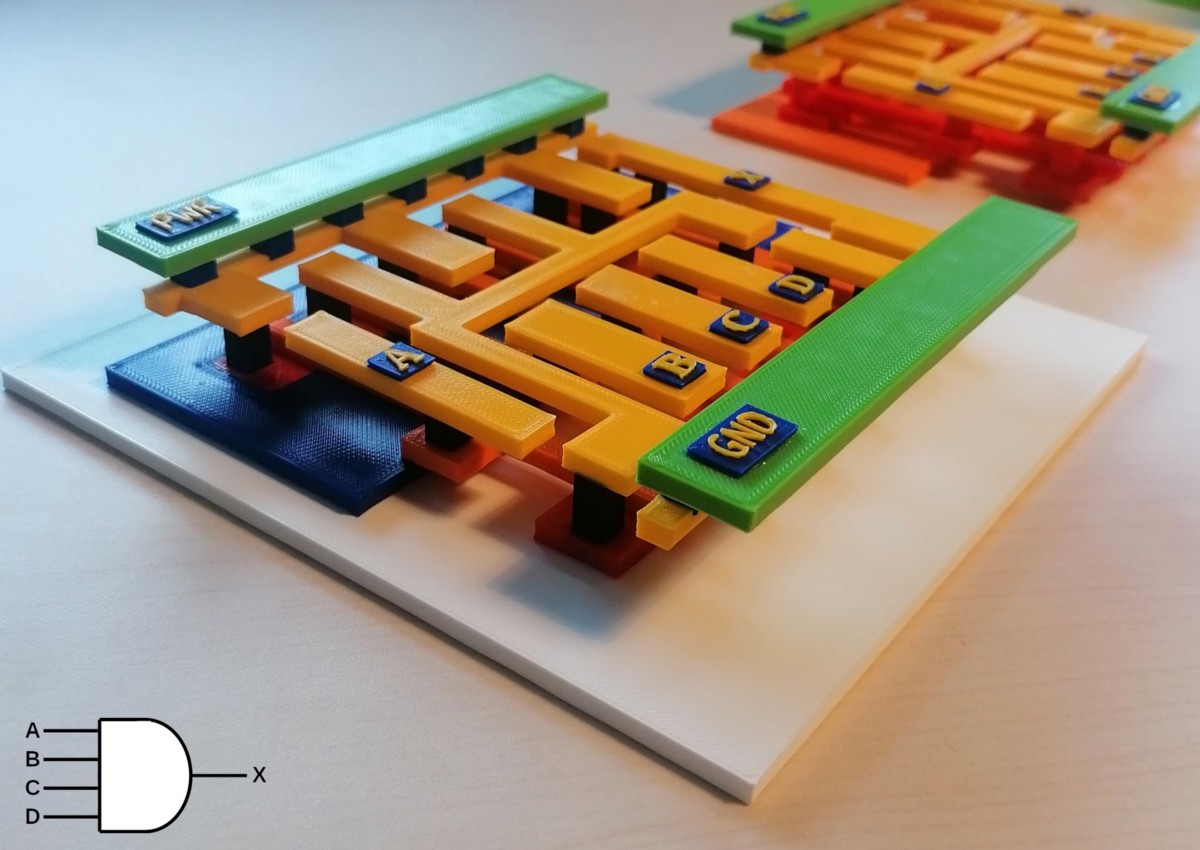
\includegraphics[width=0.4 \textwidth]{3d_and.jpeg}
	\end{center}
	\end{frame}
	
	%---------------------------------------------------------
	
	
	%---------------------------------------------------------
	%Example of the \pause command
	\begin{frame}
		\frametitle{Introduction}
		\begin{itemize}
		\item \textbf{Pre-characterization:} cells are gone through schematic design, simulations followed by Symbol creation, layout design, physical verifications, abstraction, extraction and characterization. 
		\item \textbf{Multi-drive strength cells:}drive strength of a standard cell increases when we increase the size (W/L) of its transistors.
			\begin{itemize}
				\item cells labeled as "1X", "2X", eg (BUF\_1X, BUF\_2X, and etc...)
				\item \textcolor {red} {low drive strength} cell will require less power and area but having more delay and more transition time
				\item \textcolor {red} {high drive strength} cell can drive a larger number of cells and having a fast transition.
				
			\end{itemize}
		\item \textbf{Multi-Vt cells:} Multiple threshold voltage techniques use both Low Vt and High Vt cells.
		\begin{itemize}
			\item \textbf{LVT:} \textcolor {red} {Low-Vt} cells have a lowered threshold voltage. i.e. it has a faster operation, but leakage currents are more.
			\item \textbf{HVT} \textcolor {red} {High-Vt} cells have the highest threshold voltage for device operation in this group. The cells are slower, but due to the higher threshold, leakage is also lower.
		\end{itemize}
		\end{itemize}	
	\end{frame}

	%------------------------------------------
	\begin{frame}
		\frametitle{Cell Collections}
		In general, a standard cell library contains the following types of cell:
		\begin{itemize}
			\item All basic and universal gates (like AND, OR, NOT, NAND, NOR, XOR etc)
			\item Complex gates (like MUX, HA, FA, Comparators, AOI, OAI etc)
			\item Clock tree cells (like Clock buffers, clock inverters, ICG cells etc)
			\item Flip flops and latches
			\item \textcolor {red} {Delay cells}: used to fix hold with huge magnitude of violations 
			\item \textcolor {red} {Physical only cells}
			\item Scannable Flip flops
		\end{itemize}	
		\begin{center}
		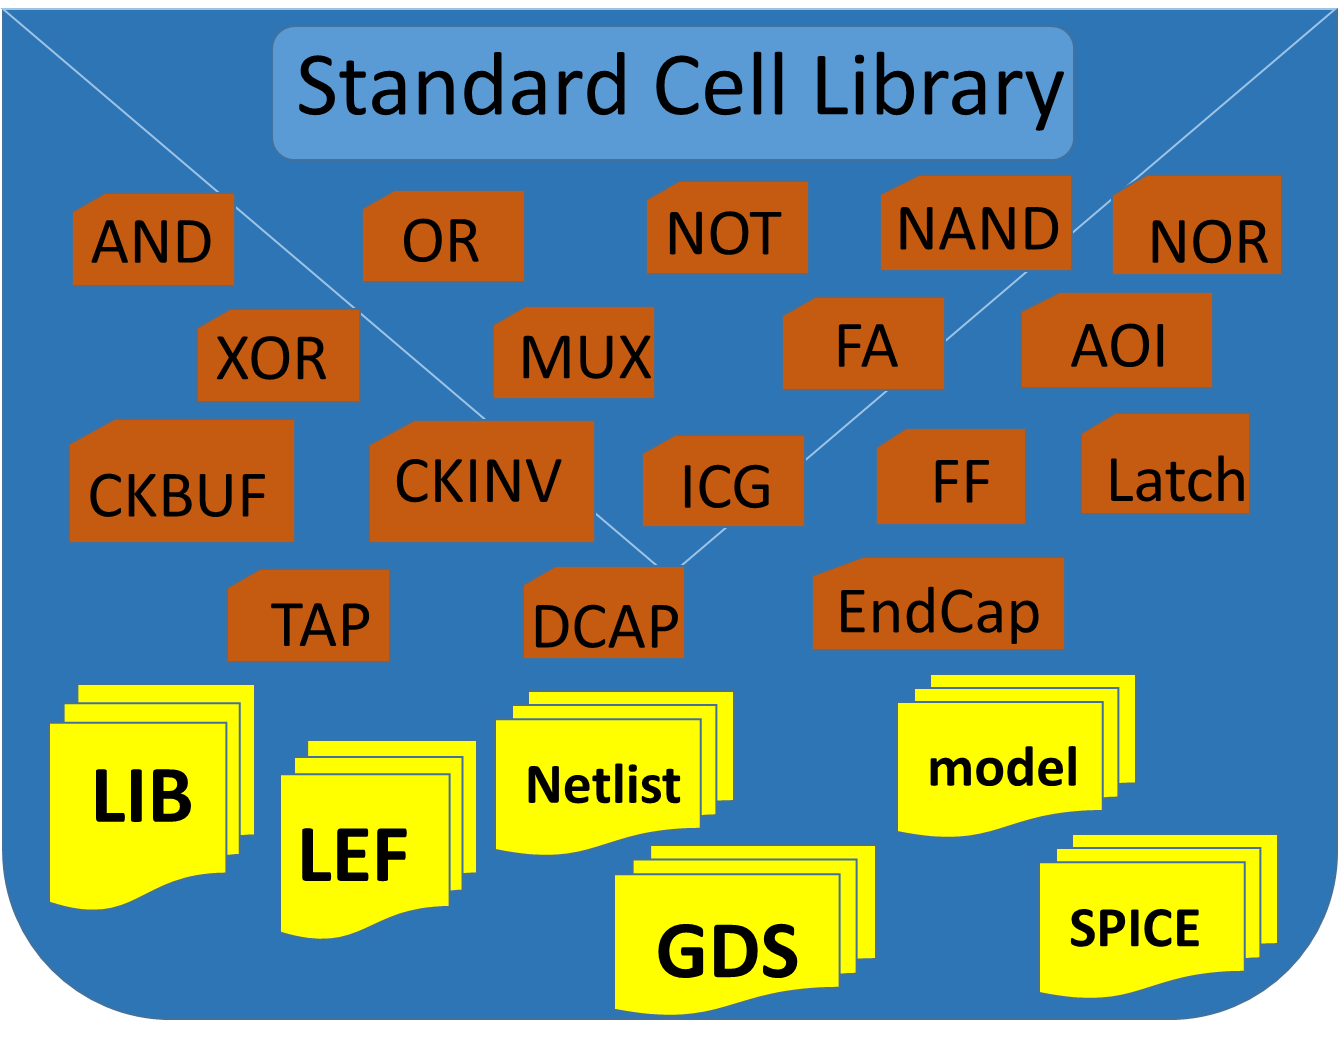
\includegraphics[width=0.35 \textwidth]{standardCellLib}
		\end{center}
	\end{frame}
	%---------------------------------------------------------
	\begin{frame}
		\frametitle{File Collections}
		Apart from the standard cells, the Standard cell library is delivered with a collection of files which contains all the information required to auto place and route. These files are mainly:
		\begin{itemize}
			\item \textcolor {red} {LIB files(.lib)}: Library files contain cell delay, power and area information
			\item \textcolor {red} {LEF files(.lef)}: LEF file contains the information of cell boundary, Pins inside the cell, location, direction, and metal layer of each pin.
			\item \textcolor {red} {Netlist file(.v )}: Netlist file is a Verilog file of the standard cell which defines the functionality of a cell.
			\item \textcolor {red} {GDS file(.gds)}: GDS file is the layout of the standard cell.
			\item \textcolor {red} {SPICE Netlist(.sp)}: SPICE netlist is the netlist of cell in SPICE format is used for simulation.
			\item \textcolor {red} {Model file(.m)}: contains the various design parameters of the cell required for SPICE simulation. 
		\end{itemize}	
	\end{frame}
%------------------------------------------------------
	\begin{frame}
	\frametitle{Standard Cell Layout}
	\begin{itemize}
		\item All the Standard cells are in equal in height and varying width.
		\item At the top of the standard cell, there is VDD rail and bottom there is a VSS rail.
		\item Both the Power rails are drawn in the Metal-1 layer.
		\item In between the VDD rail and VSS rail there are three main regions
		\begin{itemize}
			\item a nwell region, a gap of nwell and pwell and pwell region.
			\item nwell region is near to the VDD rail and pwell region is near the VSS rail.
			\item pMOS transistors are build inside the nwell, nMOS transistors are build inside the Pwell
		\end{itemize}
	\end{itemize}
		\begin{center}
	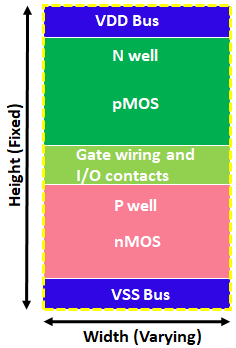
\includegraphics[width=0.2 \textwidth]{Standard_cell}\qquad \qquad
	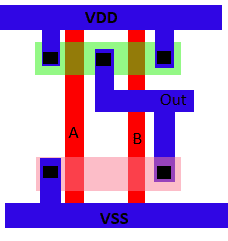
\includegraphics[width=0.2 \textwidth]{nand_layout2}

	\end{center}

\end{frame}
%----------------------------------------------
%Highlighting text
\begin{frame}
	\frametitle{Standard Cells Notes}
	
	
	\begin{block}{Remember}
		In standard cell most of the cases, the height of standard cells are constant and width varies.
	\end{block}
	
	\begin{alertblock}{Remark}
There may be double height cells, triple height cell, etc. Similarly the rows also have heights accordingly.
	\end{alertblock}
	
	\begin{examples}
	Level Shifter "is used to shift a signal voltage from one voltage domain to another" may be twice or three times as high as a standard cell with a least height.
	\end{examples}
\end{frame}
%----------------------------------------------
	\begin{frame}
	\frametitle{Exercises}
	\begin{itemize}
		\item \textcolor {red} {Why Multi-Vth Cells are required in Standard cell Library?}
		\item \textcolor {red} {If you have "HVT, SVT, and LVT"Cells Which cells would you use: }
		\begin{itemize}
			\item in order to fix setup violations.
			\item in order to fix hold violations.
			\item in Low Power Design (Power Density)
		\end{itemize}
		\item \textcolor {red} {How to implement various drive strength standard cells in fixed height?}
		\item \textcolor {red} {Compare the following cells in terms of: speed, area, and leakage power}
		\begin{itemize}
			\item svt\_x2\_buf, svt\_x8\_buf, svt\_x16\_buf
			\item svt\_x2\_buf, lvt\_x2\_buf 
		\end{itemize}
	\end{itemize}
\end{frame}
	%-------------------------------------------
	
	\section{Physical Only Cells}
	
	%---------------------------------------------------------
	%Highlighting text
	\begin{frame}
	\frametitle{Well Tap Cells}
		\begin{columns}
	
	\column{0.5\textwidth}
	\begin{itemize}
		\item Well tap cells (or Tap cells) are used to prevent the \textcolor{red} { latch-up issue} in the CMOS design.
		\item Well tap cells have no logical functions, it has only two connections
		\begin{itemize}
			\item nwell to the power supply (VDD)
			\item p-substrate to the ground (VSS)
		\end{itemize}
		\item Well tap cell has no input and output pins, therefore it is called a physical-only cell.
	\end{itemize}
	
	\column{0.5\textwidth}
	\begin{center}
		
\includegraphics[width=0.3 \textwidth]{wellTapCell}
	\end{center}
\end{columns}
\end{frame}	
%--------------------------------------------------
	\begin{frame}
	\frametitle{Why Well Tap Cell:}
	Early days there was no concept of well tap cell, Standard cells were designed in such a way that each standard cell had nwell to VDD and p-substrate to VSS connection within the standard cell.
	But such a standard cell design had consumed more area and to \textcolor{red} {save the area}, later a concept of Tapless cell has evolved. 
	In a tapless cell, there are no well taping inside the standard cell, well taping is provided by a separate standard cell which is called a well tap cell. So well tap cell is a part of a tapless standard cell library
	\begin{center}
		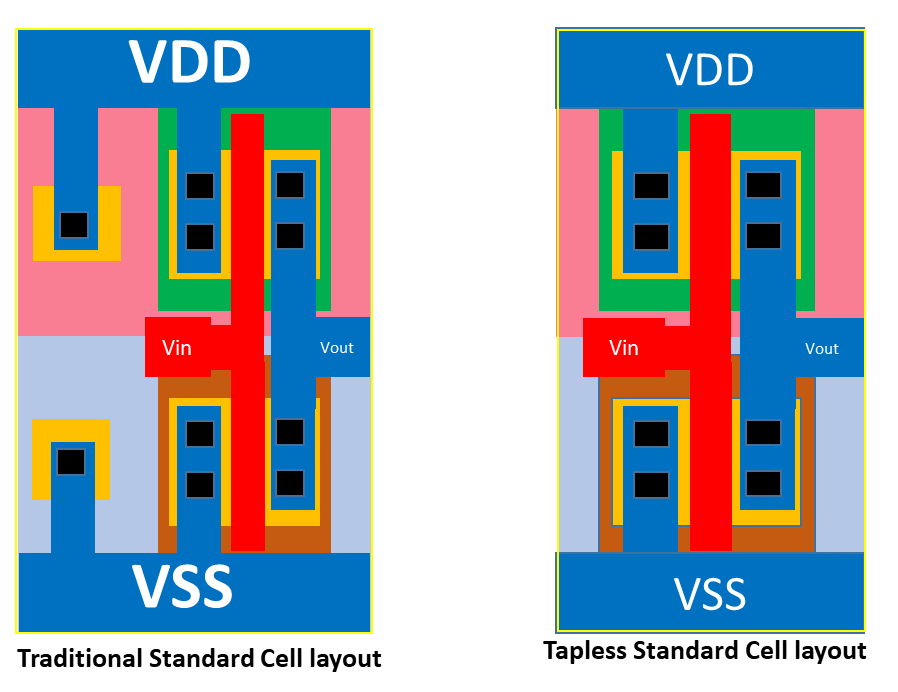
\includegraphics[width=0.4 \textwidth]{TaplessCell}
	\end{center}		
\end{frame}	

\begin{frame}
	\frametitle{Placement of  Well Tap Cells:}
	\begin{itemize}
		\item Well tap cells are placed after the macro placement and power rail creation.
		\item This stage is called the \textcolor {red} {pre-placement stage}.
		\item Well tap cells are placed in a regular interval in each row of placement.
		\item The maximum distance between the well tap cells must be as per the DRC rule of that particular technology library.
		\item If a macro comes in the path of vertical columns, then the placement of vertical column shifted alongside macro as shown in the figure.
	\end{itemize}
	\begin{center}
		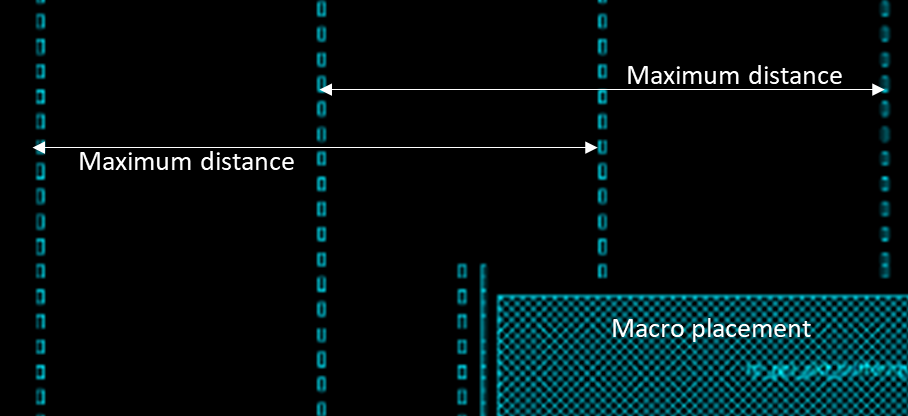
\includegraphics[width=0.4 \textwidth]{wellTapPlacement}
	\end{center}
\end{frame}
%------------------------------------------------
	\begin{frame}
	\frametitle{End Cap (Boundary) Cells}
	The end cap cells are placed in the design because of the following reasons:
	\begin{itemize}
		\item Boundary cell is placed at both the ends of each placement row to terminate the row.
		\item To protect the gate of a standard cell placed near the boundary from damage during manufacturing
		\item To avoid the base layer DRC (Nwell and Implant layer) at the boundary.
		\item It has also been placed at the top and bottom row at the block level to make integration with other blocks.
	\end{itemize}
	\begin{center}
		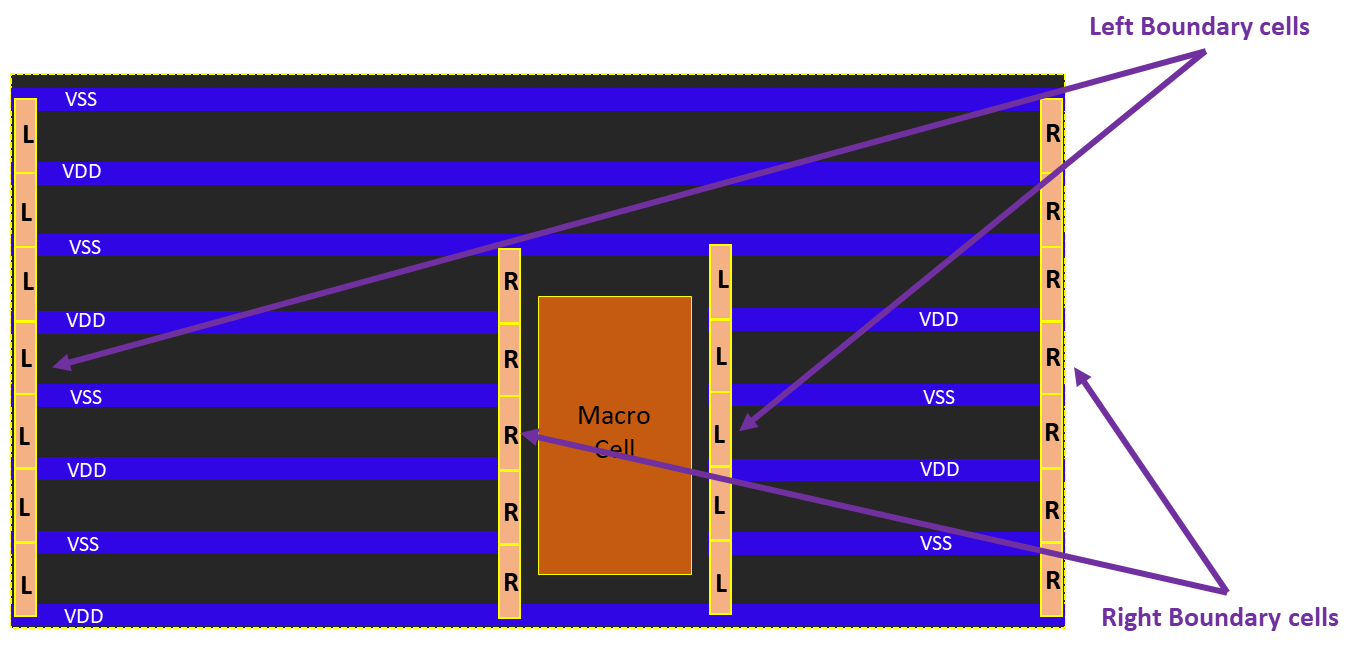
\includegraphics[width=0.45 \textwidth]{EndCapPlacement}
	\end{center}
\end{frame}	
%--------------------------------------------------------
\begin{frame}
	\frametitle{End Cap Cells Notes}
	
	\begin{block}{Remember}
		\begin{itemize}
			\item The boundary cell is a physical-only cell, has no logical functions and therefore these cells are not a part of the netlist.
			\item Boundary cells have mainly Nwell layer, implant layers, and dummy poly layer and metal rails.
		\end{itemize}
	\end{block}
	
	\begin{alertblock}{Remark}
		Boundary cells are placed just after the macro placement and site row creation. Boundary cell is placed before the placement of standard cells and therefore it is called a pre-placed cell.
	\end{alertblock}
		\begin{columns}
	\column{0.5\textwidth}
	\begin{itemize}
		\item They are also added to isolate any analog IPs and digital part of any chips.
	\end{itemize}
	
	\column{0.7\textwidth}
	\begin{center}
		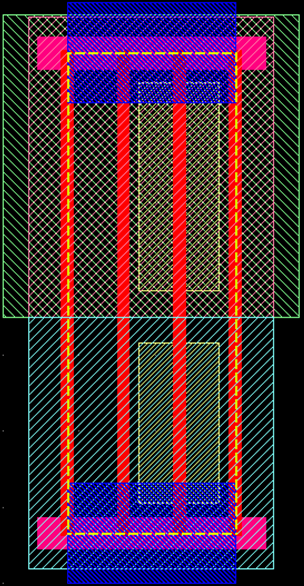
\includegraphics[width=0.15 \textwidth]{endcapCell}
	\end{center}	
\end{columns}
	
\end{frame}
%-------------------------------------------------------

	\begin{frame}
	\frametitle{DeCap Cells}
	Decap cells are basically a charge storing device made of the capacitors and used to support the instant current requirement in the power delivery network
	\begin{itemize}
		\item cells are temporary capacitors added in the design between power and ground rails to counter functional failures due to dynamic IR drop.
		\item Dynamic IR drop happens at the active edge of the clock at which a high percentage of Sequential and Digital elements switch.
		\item Due to this simultaneous switching a high current is drawn from the power grid for a small duration.
		\item If the power source is far away from a flop the chances are that this flop can go into a metastable state due to IR Drop.
		\item To overcome this decaps are added. At an active edge of clock when the current requirement is high, these decaps discharge and provide boost to the power grid.
	\end{itemize}

\end{frame}	
%--------------------------------------------------------
\begin{frame}
	\frametitle{Schematic and layout of Decap cell}
	Decap cells are typically poly gate transistors where source and drain are connected to the ground rail, and the gate is connected to the power rail.
		\begin{block}{Remember}
		\begin{itemize}
			\item Decap cells are placed generally after the power planning and before the standard cell placement, that is in the pre-placement stage.
			\item  These cells are placed uniformly throughout the design in this stage. Decap cells can also be placed in the post route stage also if required.
		\end{itemize}
	\end{block}
	\begin{center}
	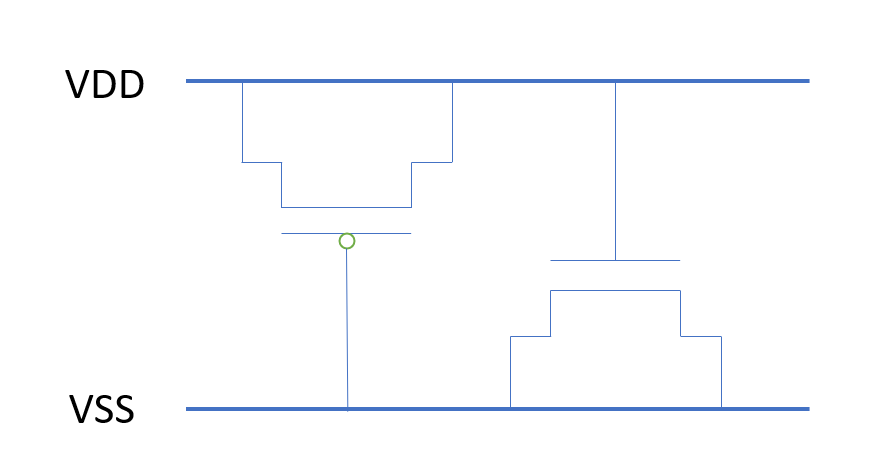
\includegraphics[width=0.3 \textwidth]{DeCap_cell}\qquad \qquad
		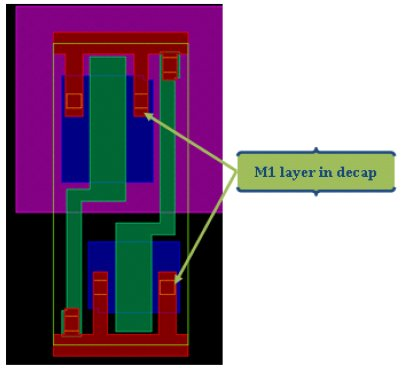
\includegraphics[width=0.3 \textwidth]{Decap_layout}
	\end{center}
\end{frame}	

\begin{frame}
	\frametitle{Tie Cells}
	\begin{itemize}
		\item The tie cell is a standard cell, designed specially to provide the high or low signal to the input (gate terminal) of any logic gate. 
		\item The high/low signal can not be applied directly to the gate of any transistors because of some limitations of transistors, especially in the lower node. 
		\item In the lower technology node, the gate oxide under the poly gate is a very thin and the most sensitive part of the transistor.
		\item It has been observed that if the polysilicon gate connects directly to VDD or VSS for a constant high/low input signal, and in case any surge/glitch arises in the supply voltage it results in damage of sensitive gate oxide.
		\item To avoid theis damages, tie cell is used to connect the input of any logic to the VDD or VSS.
	\end{itemize}
	\begin{center}
		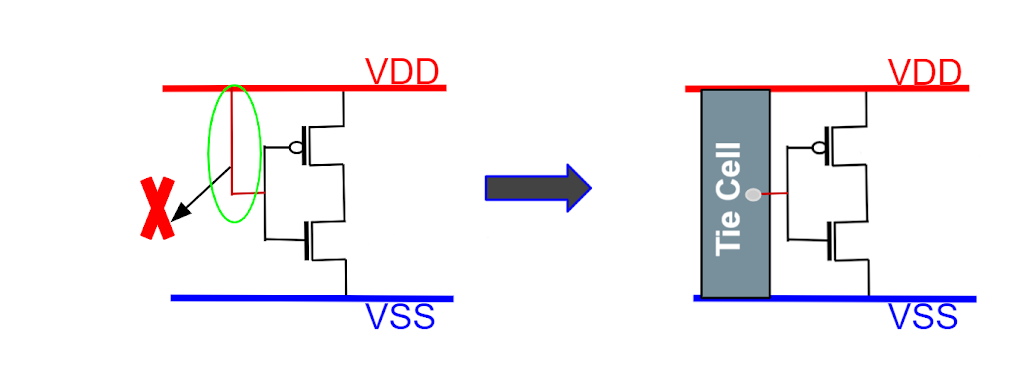
\includegraphics[width=0.4 \textwidth]{Tie_cell_need}
	\end{center}
\end{frame}	
%--------------------------------------------------------
\begin{frame}
	\frametitle{Schematic of tie cells:}
	There are two types of tie cells.
	\begin{itemize}
		\item Tie-high cell
		\item Tie-low cell
	\end{itemize}
	As the name suggests, the tie-high cell’s output is always high and the tie-low cell’s output is always low.	
	\begin{block}{Remember}
Tie cells are not present in the synthesized netlist and not placed in the initial placement of the standard cells. Tie cells are inserted in the placement stage and more specifically at the final stage of placement.
\end{block}
	\begin{center}
		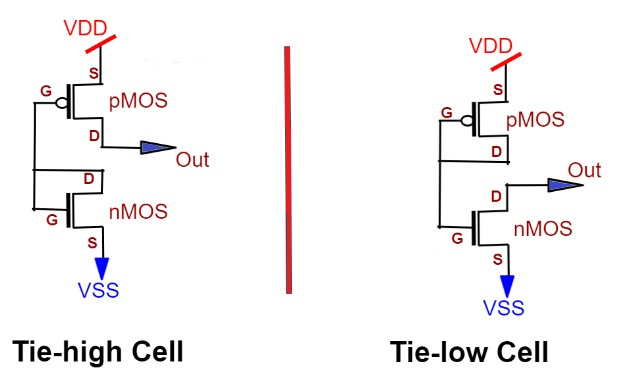
\includegraphics[width=0.4 \textwidth]{What-are-Tie-Cells-in-Physical-Design}
	\end{center}
\end{frame}	
%--------------------------------------------------------
\begin{frame}
	\frametitle{Spare cells}
	\begin{itemize}
		\item Spare cells generally consist of a group of standard cells mainly inverter, buffer, nand, nor, and, or, exor, mux, flip flops and maybe some specially designed configurable spare cells.
		\item spare cells do not perform any logical operation in the design and act as a filler cell only.
		\item The inputs of spare cells are tied either VDD or VSS through the tie cell and the output is left floating.
		\item Input can not be left floating as a floating input will be prone to get affected by noise and this could result in unnecessary switching in space cells which leads to extra power dissipation
	\end{itemize}
	\begin{center}
		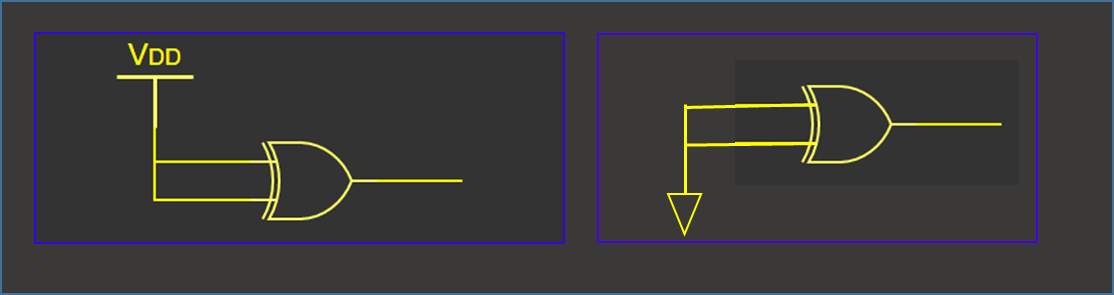
\includegraphics[width=0.3 \textwidth]{spareCellTie} \quad \quad
		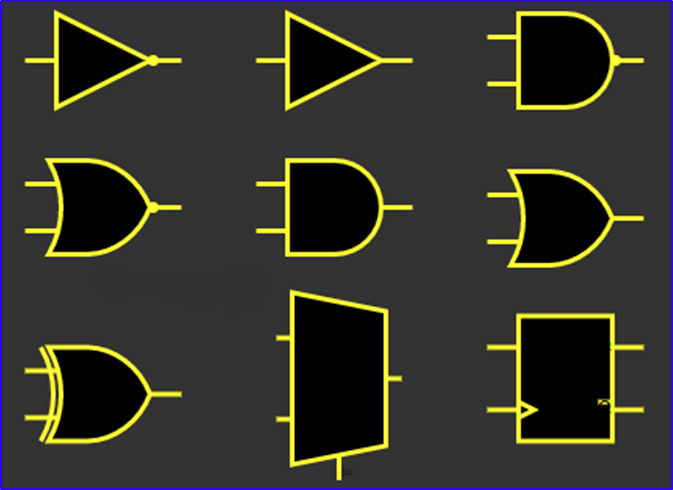
\includegraphics[width=0.3 \textwidth]{spareCell}
	\end{center}
\end{frame}	
%--------------------------------------------------------
\begin{frame}
	\frametitle{Use of Spare cells}
	\begin{itemize}
		\item Spare cells enable us to modify/improve the functionality of a chip with minimal changes in the mask. 
		\item We can use already placed spare cells from the nearby location and just need to modify the metal interconnect.
		\item There is no need to make any changes in the base layers. Using metal ECO we can modify the interconnect metal connection and make use of spare cells.
		\item We only need to change some metal mask, not the base layer masks.
	\end{itemize}
	\begin{center}
		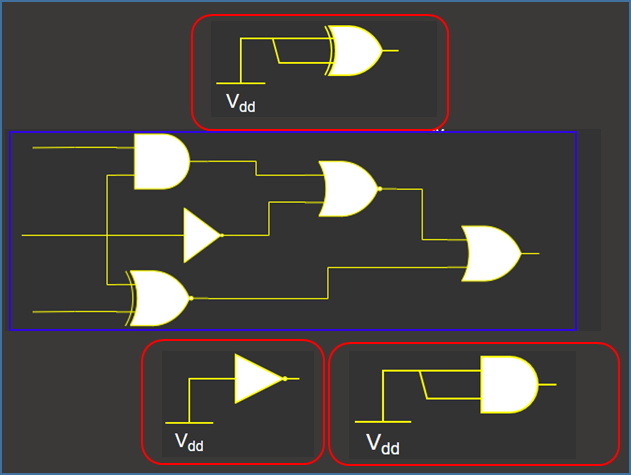
\includegraphics[width=0.3 \textwidth]{sparecellUse} 
	\end{center}
\end{frame}	
%--------------------------------------------------------
\begin{frame}
	\frametitle{Placement of Spare cells:}
	\begin{block}{Remember}
		Spare cells are added before the placement of standard cells throughout the design
	\end{block}
	
	\begin{alertblock}{Remark}
		Spare cells can be added either by the netlist or by PnR tool command.
	\end{alertblock}
	\begin{block}{Placing spare cells using ICC}
	place\_opt \\
	set physopt\_tie\_spare\_cells true \\
	insert\_spare\_cells -lib\_cell {INVX5 DFFCPX2 }\ \\
	\quad \quad -cell\_name spare -num\_instances 2 -tie -skip\_legal \\
	legalize\_placement -incremental \\
	spread\_spare\_cells [get\_cells spare*] -bbox {{30 30} {350 150}} \\
	psynopt
\end{block}
\end{frame}	
%---------------------------------------------

\begin{frame}
	\frametitle{Filler Cells}
	\begin{itemize}
		\item Once you have completed placement and routing, there are usually gaps left in the layout where you do not have any standard cells present.
		\item So, if you say you have 70\% utilization, you can expect around 30\% of the area unfilled.
		\item If you do DRC check now(in a tool that can give you base layer DRCs), you can expect to see spacing violations like “NWell minimum spacing not met”.
		\item Filler cells inserted by the P\&R tool to fill gaps in the layout after placement and routing is completed. Filler cell insertion must be completed before physical verification can begin.
	\end{itemize}
		\begin{center}
		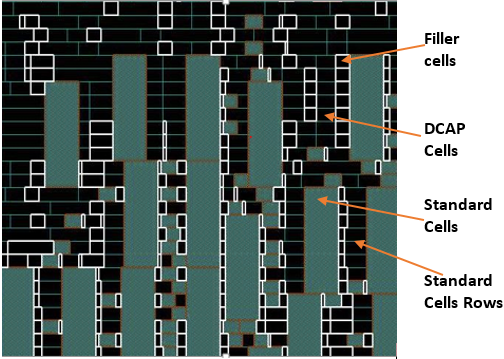
\includegraphics[width=0.3 \textwidth]{Filler} 
	\end{center}
\end{frame}	
	%---------------------------------------------------------
	\begin{frame}
		\frametitle{Filler Cells Continue...}
		\begin{itemize}	
			\item To ensure that all power nets are connected, you can fill empty space in the standard-cell rows with filler cells.
			\item Filler cells have no logical connectivity. these cells are provided continuity in the rows for VDD and VSS nets and it also contains substrate nwell connection to improve substrate biasing.
			\item Filler cell insertion is often used to add decoupling capacitors to improve the stability of the power supply and discontinuity in power
		\end{itemize}
		\begin{alertblock}{when we placed filler cells in the design}
when optimization of clock tree synthesis is completed i.e after timing has been met because let's say if we want to place buffer/inv for optimization purpose we can't place these cells because there is already placed filler cells, and enough area is not there to present buffer/inv, so after timing has been met and routing optimization is done then only placed the filler cells to fill the empty space.
	\end{alertblock}
	\end{frame}	
	
	\begin{frame}
		\frametitle{Filler Cells Continue...}
	\begin{center}
		\<بِسْمِ اللَّـهِ الرَّحْمَـٰنِ الرَّحِيمِ> \\
		 \<وَمَا أُوتِيتُمْ مِنَ الْعِلْمِ إِلَّا قَلِيلً>

	\end{center}
	\end{frame}	
\end{document}